% !TEX root = ../agglo_clust_review.tex

\begin{table*}[t]
    \centering
    \scriptsize
    % \tiny
    \begin{subtable}[t!]{\textwidth}
    \centering

        \begin{tabular}{l  c  r  c  c  | r r r r r r}
        % \toprule
        &&&& %\multicolumn{1}{c}{}
        &\multicolumn{5}{c}{Multicut objective values associated to final clusterings (lower is better)} \\
        Clustering problem & \makecell{Graph Type} & $\#I$ & $|V|$ & $|E|$  & \multicolumn{1}{r}{GAEC \cite{keuper2015efficient}} & HCC-Sum & MWS \cite{wolf2018mutex} & HC-Avg & HCC-Avg \\ \midrule
        \emph{Modularity Clustering} \cite{brandes2007modularity} & \emph{complete} & 6& 34-115 & 561-6555 & % \HollowBox & 
        -0.457 & -0.453 & -0.073 & \textbf{-0.467} & \textbf{-0.467} \\ 
        \emph{Image Segmentation} \cite{andres2011probabilistic} & \emph{rag} & 100 & 156-3764 &  439-10970  & % \HollowBox 
        \textbf{-2,955} & -2,953 & -2,901 & -2,903 & -2,896\\
        \emph{Knott-3D (150-300-450)} \cite{andres2012globally} & \emph{3D-rag} & 24 & 572-17k & 3381-107k & % \HollowBox & 
        \textbf{-36,667} & -36,652 & -35,200 & -35,957 & -35,631\\
        % \emph{Knott-3D-300} & \emph{3D-rag} & 8& & & \HollowBox\\
        % \emph{Knott-3D-450}& \emph{3D-rag} & 8 & & & \HollowBox\\  
        \emph{CREMI-3D-rag (OurCNN)}  & \emph{3D-rag} & 3& 134k-157k & 928k-1065k % & \CrossedBox 
        & \textbf{-1,112,287} & -1,112,286& -1,109,731 & -1,112,177 & -1,112,100\\ 
        \emph{Fruit-Fly Level 1-4} \cite{pape2017solving} & \emph{3D-rag} & 4& 5m-11m & 28m-72m %& \HollowBox 
        & \textbf{-151,022} & -151,017 & -150,879 & -150,909 & -150,876\\
        \emph{CREMI-gridGraph (OurCNN)} & \emph{gridGraph} & 15& 39m & 140m %& \CrossedBox 
        & -73,317,601 & -73,328,867 & -73,330,568 & \textbf{-73,502,947} & -73,474,856\\
        \emph{Fruit-Fly Level Global} \cite{pape2017solving} & \emph{3D-rag} & 1& 90m & 650m % & \HollowBox 
        & \textbf{-151,688} & -151,596 & -146,315 & -150,466 & -150,171 \\
        % \emph{(CREMI-pixGrid-LSIMasksUNet)} & \emph{gridGraph} & 1 & & 4 & \CrossedBox\\
        % \emph{(CityScapesValidation-pixGrid)} & \emph{gridGraph} &  &  & & \CrossedBox\\
        % \emph{CREMI-test....}\\\midrule
        % \emph{Stochastic Block Model (synthetic)} & \emph{non-planar} &-&- & - & \CrossedBox \\
        % \emph{(epinions and slashdot?)} & \emph{dense?} &  & & & \HollowBox\\ 

% % Superpixels:
% Mutex & -1109731264 \\
% MEANconstr & -1112099691 \\
% MEAN & -1112176981 \\
% SUMconstrNoLogs & -1112286144 \\
% SUMnoLogs & -1112286741 \\
% Agglo type & multicut_energy \\

% % Pixels:
% SUM & -73317601 \\
% SUMconstr & -73328867 \\
% MutexPixGrid & -73330568 \\
% MEANconstr & -73474856 \\
% MEAN & -73502947 \\

        \end{tabular}
    \end{subtable} 
    \caption{List of compared signed graph clustering problems: for each, we specify the number of instances $\# I$, number of nodes $|V|$, and number of edges $|E|$. We compare algorithms in the \algname{} framework by evaluating which of the obtained clusterings is associated to the lowest value of the multicut objective defined in Eq.~\ref{eq:MC_objective} (lower is better).} 
    \label{tab:datasets_and_energies}
\end{table*}


\section{Experiments}\label{sec:neuro_segm_exp}
\subsection{Signed graph clustering problems}
We evaluate the agglomerative clustering algorithms included in our framework on a large collection of both synthetic and real-world graphs. The size of the graphs ranges from a few hundred to hundreds of millions of edges and the graphs have very different structures, so that the algorithms are tested in very different scenarios.

\textbf{Synthetic SSBM graphs} -- We first consider synthetic graphs generated by a signed stochastic block model (SSBM). We use an Erd\H os-R\'enyi random graph model $\mathcal{G}(N,p)$ with $N$ vertices and edge probability $p$. Following the approach in \cite{Cucuringu2019SPONGEAG}, we partitioned the graph into $k$ equally-sized clusters, such that edges connecting vertices belonging to the same cluster (different clusters, respectively) have Gaussian distributed edge weights centered at $\mu=1$ ($\mu=-1$, respectively) and with standard deviation $\sigma=0.1$. To model noise, the sign of the edge weights is flipped independently with probability $\eta$.


\textbf{Existing signed graphs}  -- We use clustering instances from the OpenGM benchmark \cite{kappes2013comparative} as well as biomedical segmentation instances \cite{pape2017solving}. The dataset \emph{Image Segmentation} contains planar region-adjacency-graphs (\emph{rag}) that are constructed from superpixel adjacencies of photographs. The \emph{Knott-3D} datasets contains \emph{3D-rags} arising from volume images acquired by electron microscopy (EM). The set \emph{Modularity Clustering} contains complete graphs constructed from clustering problems on small social networks. The \emph{Fruit-Fly} 3D-rag instances were generated from volume image scans of fruit fly brain matter. Instances \emph{Level 1-4} are progressively simplified versions of the global problem obtained via block-wise domain decomposition \cite{pape2017solving}.

\textbf{Grid-graphs from CNN predictions} -- We also evaluate the clustering methods on the task of neuron segmentation in EM image volumes using training data from the CREMI 2016 EM Segmentation Challenge \cite{cremiChallenge}.
We train a 3D U-Net \cite{ronneberger2015u,cciccek20163d} using the same architecture as \cite{funke2018large} and predict long-and-short range affinities 
as described in \cite{lee2017superhuman}\footnote{See Appendix \ref{sec:cremi_details} for all details about training and data augmentation.}. The predicted affinities $a_e\in[0,1]$, which represent how likely it is for a pair of pixels to belong to the same neuron segment, are then mapped to signed edge weights $w_e=a_e-0.5$, resulting in a 3D grid-graph having a node for each pixel/voxel of the  image\footnote{To map affinities to signed weights, we also tested the \emph{logarithmic mapping} proposed in \cite{finkel2008enforcing,andres2012globally}, but it performed worse in our experiments.}. 
Clustering algorithms largely benefit from long-range edge connections in the grid-graph, in addition to direct-neighbors ones. However, empirically, we found that long-range affinities predicted by the CNN are also more noisy, and adding only 10\% of them (by random sampling) gave the best results.
% \TODO{long-range 10\%} 
% Adding long-range connections to the graph is generally helpful, but when many of them carry repulsive weights. Long-range connections are more noisy. 10\% represents a good compromise.
We divided the three CREMI training samples, consisting of $\sim$196 million voxels each, into five sub-blocks for a total of 15 clustering problems (named \emph{CREMI-gridGraph} in Table~\ref{tab:datasets_and_energies}). 

\textbf{3D-rag from CNN-predictions} -- Lastly, we use the predictions of our CNN model to generate three graph instances (one for each CREMI training sample, named \emph{CREMI-3D-rag} in Table~\ref{tab:datasets_and_energies}), which have very similar structure to the \emph{Knott-3D} and \emph{Fruit-Fly} instances.  We obtain them by first computing 2D supervoxels from the CNN predictions (using a watershed algorithm seeded at the maxima of the smoothed boundary distance transform) and then building a 3D region-adjacency graph, whose edge weights are given by the CNN affinities averaged over the boundaries of adjacent supervoxels.

% This is true for the neuron instances generated from the CREMI challenge, where training data is available, and for synthetic graphs generated with SSBM.   


% Fig.~\ref{fig:noise_plots} summarizes our 12000 noise experiments: we focus on the best performing linkage criteria, i.e. \emph{Average}, \emph{Sum} and \emph{Abs Max}, and test them with different amount of noise. 
% In these experiments, we also want to assess how beneficial it is to use long-range CNN predictions in the agglomeration. Thus, we perform a set of simulations without adding long-range connections to the grid-graph and another set where we introduce them with a 10\% probability\footnote{We also performed experiments adding all the long-range predictions given by the CNN model, but we did not note major differences when using only 10\% of them. Adding this fraction is usually sufficient to improve the scores.}.\\



% , where $\beta \in [0,1]$ is a \emph{bias} parameter that allow a tuning between over- and under-segmentation and in our case was set to $\beta=0.5$.
% Neuron segmentation is commonly performed by first predicting undirected affinities \cite{wolf2018mutex,lee2017superhuman,funke2018large}, which represent how likely it is for a pair of pixels to belong to the same neuron segment. 
% Similarly to \cite{lee2017superhuman}, we train a UNet model CITE to predict both short- and long-range affinities that are not limited to adjacent pixels. These predictions are then used as edge weights of a 3D grid graph, where each node represents a pixel/voxel of the volume image. 
 


% ---
% We first evaluate and compare the agglomerative clustering algorithms described in the generalized framework on the task of neuron segmentation in electron microscopy (EM) image volumes. This application is of key interest in connectomics, a field of neuro-science with the goal of reconstructing neural wiring diagrams spanning complete central nervous systems. Currently, only proof-reading or manual tracing yields sufficient accuracy for correct circuit reconstruction \cite{schlegel2017learning}, thus further progress is required in automated reconstruction methods.





% ----
% We evaluate all algorithms in the proposed framework on the competitive CREMI 2016 EM Segmentation Challenge \cite{cremiChallenge} that is currently the neuron segmentation challenge with the largest amount of training data available. The dataset comes from serial section EM of \emph{Drosophila} fruit-fly tissue and consists of 6 volumes of 1250x1250x125 voxels at resolution 4x4x40nm, three of which come with publicly available training ground truth. The results submitted to the leaderboard are evaluated using the CREMI score, based on the Adapted Rand-Score (Rand-Score) and the Variation of Information Score \cite{arganda2015crowdsourcing}. In Appendix \ref{sec:cremi_details}, we provide more details about the training of our CNN model, inspired by work of \cite{lee2017superhuman,funke2018large}.



\begin{table*}[t]
        \centering
% \begin{minipage}[t]{0.6\textwidth}
%     \centering
    \tiny
        \begin{subtable}[t]{0.29\textwidth}
        \centering
        \begin{tabular}[t]{lcccc}
        \toprule
          & \makecell{ARAND\\error} & \makecell{VOI\\split} & \makecell{VOI\\merge}&  \makecell{Runtime\\(s)} \\ \midrule 
\textbf{HC-Avg} & \textbf{0.0487} & 0.387 & 0.258 & 2344 \\
HCC-Avg & 0.0492 & 0.389 & 0.259 & 2892 \\
MWS \cite{wolf2018mutex} & 0.0554 & 0.440 & 0.249 & 688 \\
GAEC \cite{keuper2015efficient} & 0.0856 & 0.356 & 0.338 & 4717 \\
HCC-Sum & 0.0872 & 0.365 & 0.337 & 4970 \\
HCC-Complete & 0.9206 & 4.531 & \textbf{0.210} & 1330 \\
HC-Complete & 0.9211 & 4.536 & 0.211 & 1020 \\
HC-Single & 0.9264 & \textbf{0.060} & 4.887 & \textbf{312} \\
HCC-Single & 0.9264 & \textbf{0.060} & 4.887 & 6440 \\
% HC-Avg & \textbf{0.226}  \\
% HCC-Sum & 0.282 \\
% MWS \cite{wolf2018mutex} & 0.322 \\
% GAEC \cite{keuper2015efficient} & 0.334 \\
% HCC-Avg & 0.563 \\
% HC-Single & 1.521 \\ 
% HCC-Single & 0.324 \\
% HC-Complete & 1.521 \\ 
% HCC-Complete & 1.521 \\ 
        \end{tabular}
    % \captionof{table}{CREMI-Scores achieved by different linkage criteria and thresholding. All methods use the affinity predictions from our CNN as input. Scores are averaged over the three CREMI training datasets.}
    \caption{\emph{CREMI-gridGraph (OurCNN)}}
    \label{tab:scores_gridGraph}
    \centering
    \tiny
    \end{subtable}\hfill
\begin{subtable}[t]{.29\textwidth}
\centering
        \begin{tabular}[t]{lcccc}
        \toprule
          & \makecell{ARAND\\error} & \makecell{VOI\\split} & \makecell{VOI\\merge}&  \makecell{Runtime\\(s)} \\ \midrule 
\textbf{HC-Avg} & \textbf{0.0896} & 0.603 & 0.323 & 86 \\
HCC-Avg & 0.0898 & 0.600 & 0.325 & 87 \\
GAEC \cite{keuper2015efficient} & 0.0905 & 0.606 & 0.323 & 89 \\
HCC-Sum & 0.0910 & 0.608 & 0.323 & \textbf{85} \\
MWS \cite{wolf2018mutex} & 0.1145 & 0.825 & 0.295 & 86 \\
HCC-Single & 0.5282 & \textbf{0.437} & 1.367 & 88 \\
HC-Single & 0.5282 & \textbf{0.437} & 1.367 & \textbf{85} \\
HCC-Complete & 0.5564 & 2.220 & 0.254 & 89 \\
HC-Complete & 0.5654 & 2.253 & \textbf{0.249} & 86 \\
        \end{tabular}
        \hspace*{5em}
    \caption{\emph{CREMI-3D-rag (OurCNN)}}
    \label{tab:scores_3drag}
    \end{subtable}\hfill
    \begin{subtable}[t]{.38\textwidth}
    % \end{table}
% \end{minipage}\hfill
% \begin{minipage}[t]{0.38\textwidth}
    \centering
    \tiny
        \begin{tabular}[t]{lcccc}
        \toprule
          & \makecell{CREMI\\Score} & \makecell{ARAND\\error} & \makecell{VOI\\split} & \makecell{VOI\\merge}    \\ \midrule 
OurCNN: 3D-rag + LiftedMulticut & \textbf{0.221} & \textbf{0.108} & \textbf{0.339} & 0.115 \\
\emph{OurCNN: gridGraph + HCC-Avg} & 0.224 & 0.113 & 0.361 & 0.085  \\
\emph{OurCNN: gridGraph + HC-Avg}  & 0.224 & 0.114 &  0.364 & 0.083 \\
PNI CNN \cite{lee2017superhuman} & 0.228 & 0.116 & 0.345 & 0.106 \\
LSI-Masks \cite{bailoni2020proposal}  & 0.246 & 0.125 & 0.383 & 0.107  \\
\emph{OurCNN: 3D-rag + HCC-Avg} & 0.257 & 0.132 & 0.438& \textbf{0.063} \\  
\emph{OurCNN: 3D-rag + HC-Avg} & 0.262 & 0.135 & 0.448 & \textbf{0.063}   \\  
% \textbf{Our CNN + \algname{} Average} & \textbf{0.241 \\
MALA CNN + MC \cite{funke2018large} & 0.276  & 0.132 &0.490  & 0.089  \\
CRU-Net \cite{zeng2017deepem3d} & 0.566 & 0.229 & 1.081 &  0.389    \\
% LFC \cite{parag2017anisotropic} & 0.616 & 0.313 & 1.085 & 0.140     \\
        \end{tabular}
        \caption{CREMI Challenge leader-board}
        \label{tab:cremi_leaderboard}
        \end{subtable}
        % \vspace*{0.99em}
    % \captionof{table}{Current leading entries  in the CREMI challenge leaderboard \cite{cremiChallenge} (March 2021)}
    % \label{tab:results_cremi_test}
    \caption{\textbf{Tables (a-b)}: Scores and run times of algorithms in the \algname{} framework on the \emph{CREMI-gridGraph} and \emph{CREMI-3D-rag} clustering problems: average linkage methods performed best. Measures shown are: Adapted-Rand error (ARAND, lower is better); Variation of Information (VOI) \cite{arganda2015crowdsourcing} (VOI-merge for under-clustering error and VOI-split for over-clustering error, lower values are better). \textbf{Table (c)}: Current leading entries in the CREMI challenge leaderboard (March 2021). CREMI-score is given by geometric mean of (VOI-split + VOI-merge)  and adapted RAND error (lower is better).}
    \label{tab:scores}
% \end{minipage}
\end{table*}

\subsection{Comparison results and discussion}
% Before to evaluate the clustering algorithms on real-world graphs, we compare them on two types of synthetically generated graphs and highlight some of their fundamental properties.

\textbf{Multicut objective values} -- In Table~\ref{tab:datasets_and_energies}, we report the values of the multicut objective associated to the clusterings obtained with different \algname{} algorithms\footnote{Objective values achieved by Single and Complete linkage methods are much worse compared to other algorithms and are reported in Table \ref{tab:extended_results_cremi}, in Appendix.}. Although a lot of heuristics were proposed to better optimize this objective \cite{beier2016efficient,beier2014cut,kernighan1970efficient}, these methods are out of the scope of this paper, since they do not scale up to the largest graph instances considered here. By looking at results in Table~\ref{tab:datasets_and_energies}, we observe that GAEC almost always achieves the lowest objective values, apart from the \emph{CREMI-gridGraph} instances. Despite this, on graphs where a GT clustering is known, GAEC does not achieve the best ARAND scores (see Tables~\ref{tab:scores_gridGraph} and \ref{tab:scores_3drag}). 
% To better understand these empirical results, we now make the following important observation.
% This can also be observed in our experiments on synthetic graphs (Fig. ? and ?), where the clustering with minimum multicut energy become very different from the ground truth clustering when the flip noise parameter $\eta$ is increased.

\textbf{Size of growing clusters: Sum vs Avg linkage} --
In all the studied clustering problems, we empirically observe that sum-linkage algorithms like GAEC tend to grow clusters one after the other, as shown in Fig.\ \ref{fig:intro_figure} and \ref{fig:dendrograms} by the unique agglomeration order of GAEC\footnote{This \emph{flooding agglomeration-strategy} of GAEC was also observed in \cite{kardoostsolving}.}. This is intuitively explained by the  following: initially, many of the most attractive edge weights have very similar values; when the two nodes $u,v$ with the highest attraction are merged, there is a high chance that they will have a common neighboring node $t$ belonging to the same cluster; thus, the interaction between the merged nodes $uv$ and $t$ is likely assigned to the highest priority, because it is given by the sum of two highly attractive edge weights. This will then start a ``chain reaction'' where only a single cluster is agglomerated at the time. 
% This \emph{flooding strategy} in the agglomeration is not observed with other linkage methods, e.g. Average, which grow clusters of similar sizes in parallel.
In the following, we will show how this unique \emph{flooding strategy} of the sum-linkage methods can be both an advantage or a disadvantage, depending on the type of clustering problem. 

\textbf{Comparison to spectral clustering} -- 
The spectral clustering methods for signed graphs SPONGE$_{sym}$ and SPONGE proposed by \cite{Cucuringu2019SPONGEAG} achieved state of the art performances on SSBM synthetic graphs. Their competitive performances are also confirmed by our experiments in Fig.~\ref{fig:SSBM_scores}.
% First, we compare \algname{} to spectral clustering methods for signed graphs. 
% In Fig.~\ref{fig:SSBM_scores}, we see that SPONGE$_{sym}$ and SPONGE proposed by \cite{Cucuringu2019SPONGEAG} perform particularly well on synthetic graphs generated with a SSBM. 
However, these methods do not scale up to the large graph instances considered here and they also require the user to specify the true number of clusters in advance, which is not known for other graph instances tested in this paper. In Appendix, Table \ref{tab:cremi_spectral_experiments}, we report the scores achieved by these methods on a much smaller sub-instance of the \emph{CREMI-gridGraph} problem: even when the true number of clusters is specified in advance for the spectral methods, they perform much worse than other \algname{} algorithms, with performance drop of almost 50\%. For these reasons, we exclude them from our other comparison experiments.  

\textbf{GASP on synthetic SSBM graphs}  -- 
% can be connected to any  that, depending on the edge-probability parameter $p$, are also \emph{dense}. 
\algname{} algorithms using cannotLinkConstraints are not expected to perform well on these graphs, because of the type of employed flip noise, so we focus our comparison only on the GAEC, HC-Avg and MWS algorithms (using Sum, Average, and AbsMax linkage methods, respectively).
Empirically, we observe that GAEC is the agglomerative algorithm performing best on SSBM graphs, almost as good as the spectral method SPONGE$_{sym}$ (see Fig.~\ref{fig:SSBM_scores}). Given the simple properties of SSBM graphs, we will now give a specific explanation of these empirical results. 
In SSBM graphs, the number of edges $E_{ij}\equiv(S_i\times S_j)\cap E$ connecting two clusters $S_i,S_j$ is  proportional to the product $|S_i|\cdot|S_j|$ of cluster sizes. 
With Sum or Avg linkage methods, due to the law of large numbers, the flipping noise is ``averaged out'' as soon as the set $E_{ij}$ becomes larger and clusters grow in size.
On the other hand, when clusters are small, it is more likely that several of the edges in $E_{ij}$ are flipped and the algorithm makes a mistake by merging two clusters belonging to different ground truth communities. From this observation, it follows that the \emph{flooding strategy} of the sum-linkage algorithm GAEC is a very good strategy on these types of graphs, because clusters are immediately grown in size (see dendrograms in Fig.~\ref{fig:dendrograms}). Average linkage method HC-Avg instead performs much worse on these graphs because it grows small equally-sized clusters and makes several wrong merge-decisions at the beginning. 
% This observation also explains the empirical results of \cite{chehreghani2020hierarchical}, which involved graph instances with very similar structure to the ones considered here. 
Lastly, the MWS algorithm is not expected to perform well on these graphs because of the high sensitivity of the AbsMax linkage to flipping noise. In Propositions \ref{prop:MWS_SSBM_1} and \ref{prop:MWS_SSBM_2} (see Appendix), we prove that on SSBM graphs the merging steps of the MWS algorithm are given by a sequence of ``coin flip'' decisions with a probability proportional to the noise parameter $\eta$, independently on the cluster sizes.

\textbf{Complete and Single Linkage} -- We use these two linkage methods as baselines to highlight the difficulty of the studied graph clustering problems listed in Table~\ref{tab:datasets_and_energies}. Scores in Tables~\ref{tab:scores_gridGraph}-\ref{tab:scores_3drag} show their poor performances: Single linkage hierarchical clustering (HC-Single), which here is equivalent to thresholding the edge weights at $w_e=0$ and computing connected components in the graph, often returned few big under-segmented clusters. HC-Complete and HCC-Complete returned instead a lot of over-segmented clusters. 
% These algorithms are excluded from our next comparison experiments.




\begin{figure}[t]
\begin{subfigure}[t]{0.23\textwidth}
\centering
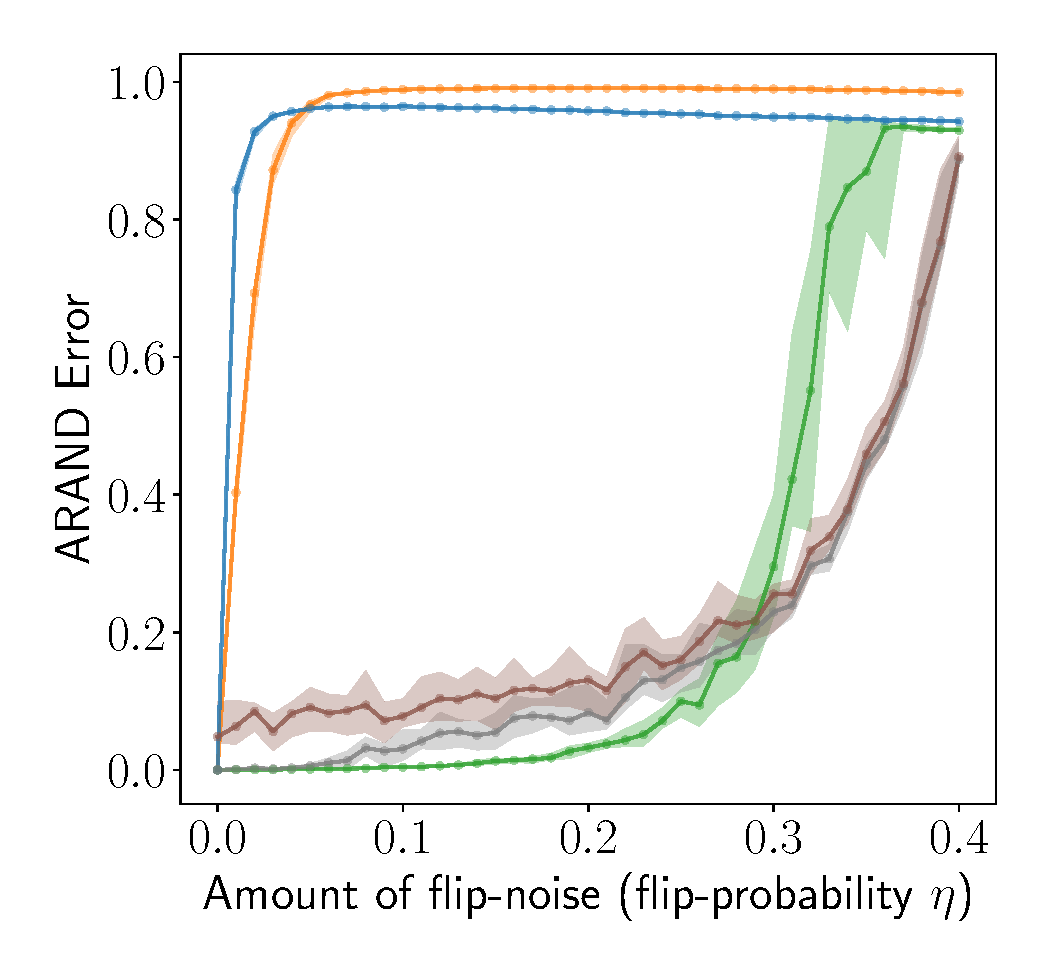
\includegraphics[width=\textwidth,trim=0.34in 0.34in 0.34in 0.34in,clip]{./figs/SSBM_scores/summary_SSBM_experiments_k20.pdf}
\caption{$k=20$, $p=0.1$}
\end{subfigure}\hfill
\begin{subfigure}[t]{0.23\textwidth}
\centering
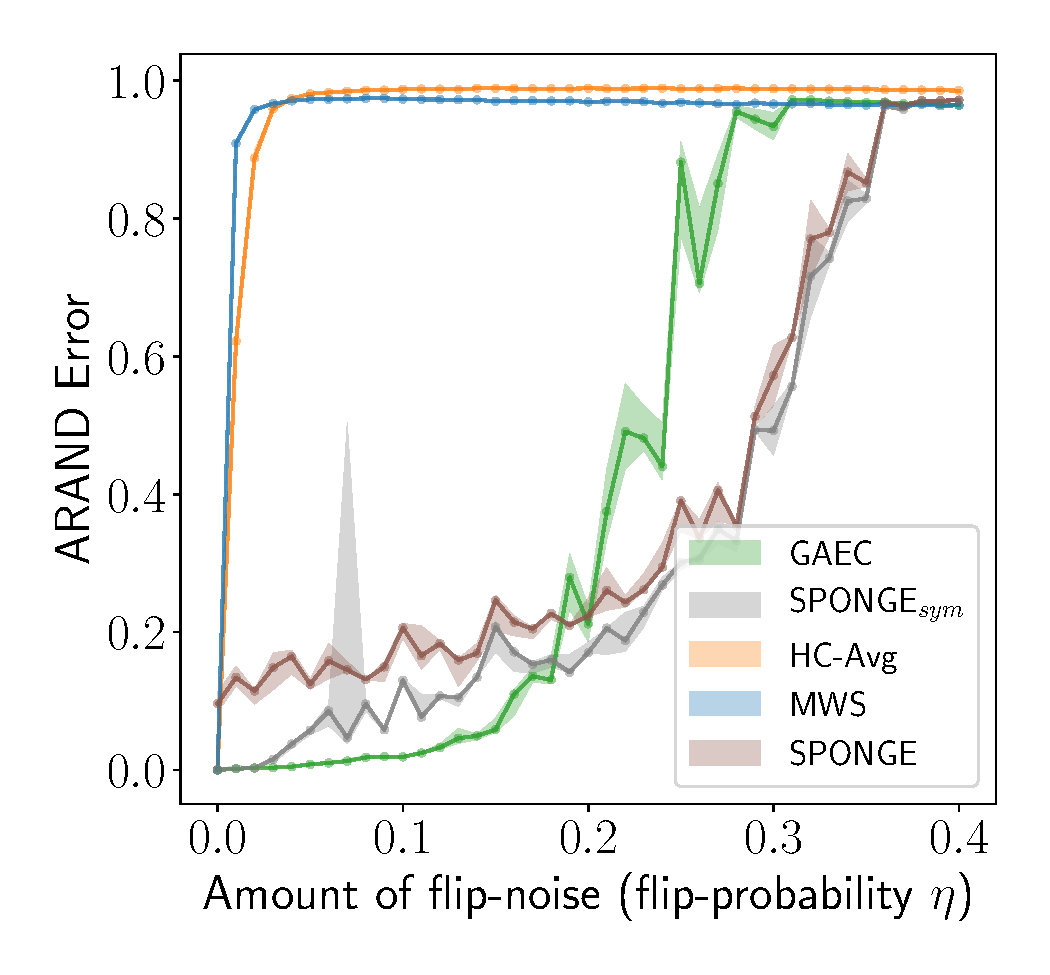
\includegraphics[width=\textwidth,trim=0.34in 0.34in 0.34in 0.34in,clip]{./figs/SSBM_scores/summary_SSBM_experiments_k50.pdf}
\caption{$k=50$, $p=0.2$}
\end{subfigure}
        \caption{
ARAND errors (median values over 20 experiments, lower is better) on synthetic graphs generated with SSBM, with $N=10000$ nodes, edges added with probability $p$, and $k$ ground truth communities of random size. 
% The spectral clustering methods, SPONGE and SPONGE$_sym$, were given the true number of clusters as input. 
% Solid lines represent median values over \TODO{30} experiments. Values between the 25th and the 75th percentile are shown in shaded areas.
% We report median, 25th, and the 75th percentile values over \TODO{30} experiments.
%         Scores on SSBM graphs
% \algname{} sensitivity to noise: \emph{Average} linkage proved to be the most robust. Performances are given by Rand-Score (higher is better) depending on the amount of noise added to the CNN predictions.  The two sets of experiments using under- and over-clustering noise are summarized in the plots at the top and at the bottom, respectively (see Appendix \ref{sec:appendix_noise_gen} for more details). For each experiment, some of the long-range CNN predictions were randomly selected with probability $p_{\mathrm{long}}$ and added as long-range edges to the pixel grid-graph. Experiments are performed on a crop of CREMI training sample B.
        } \label{fig:SSBM_scores}
\end{figure}





 



\textbf{Scores on CREMI instance-segmentation} -- 
SSBM graphs are \emph{non-planar} graphs, where every edge has the same probability to be present. On the other hand, the \emph{gridGraph} and \emph{3D-rag} graphs of Table~\ref{tab:datasets_and_energies} are sparse and have a very regular structure: weather a node represents a pixel or a superpixel, it will only have edge connections with its neighbors in the image (up to a certain hop distance). 
Tables~\ref{tab:scores_3drag}-\ref{tab:scores_gridGraph} show that average linkage methods (\emph{HC-Avg}, \emph{HCC-Avg}) strongly outperforms other methods on \emph{CREMI-gridGraph} instances and also achieves the best scores on \emph{CREMI-3D-rag} graphs. Sum-based linkage methods (\emph{GAEC}, \emph{HCC-Sum}) do not perform well on grid-graphs and often return under-clustered segments (see failure cases in Fig.~\ref{fig:failure_cases}). This suggests that the \emph{flooding strategy} observed previously in the sum-linkage methods does not work well on grid-graphs, because of the sparse local edge connections with strongly spatially-correlated noise (given that edge weights are predicted by a CNN)\footnote{This effect is not as strong on \emph{3D-rag} graphs, because edge weights are computed by averaging CNN predictions (and noise) over the boundaries of adjacent supervoxels.}.
To fully test this hypothesis, we conduct a set of experiments where the CNN predictions are perturbed by adding structured noise and simulating additional artifacts like ``holes'' in the boundary evidence\footnote{See Appendix \ref{sec:appendix_noise_gen} for details about how we perturbed the \emph{CREMI-gridGraph} problems by using Perlin noise \cite{perlin2001noise,perlin1985image}, which is one of the most common gradient noises used in procedural pattern generation.}. 
The plot in Fig.~\ref{fig:scores_structured_noise} confirms that \emph{HC-Avg} and \emph{HCC-Avg} perform well even in the presence of strong structured noise, followed by Sum-linkage algorithms and the Mutex Watershed algorithm (\emph{MWS}). It is not a surprise that the AbsMax linkage used by \emph{MWS} is not robust to this type of structured noise. However, the scores and runtimes in Table~\ref{tab:scores_gridGraph} prove how \emph{MWS} can achieve competitive performances with considerably lower runtimes. 

\begin{figure}
\centering
% \includegraphics[width=0.48\textwidth,trim=300 100 300 100, clip]{./figs/dendrograms/new_agglo_order_OLD.png} % left bottom right top
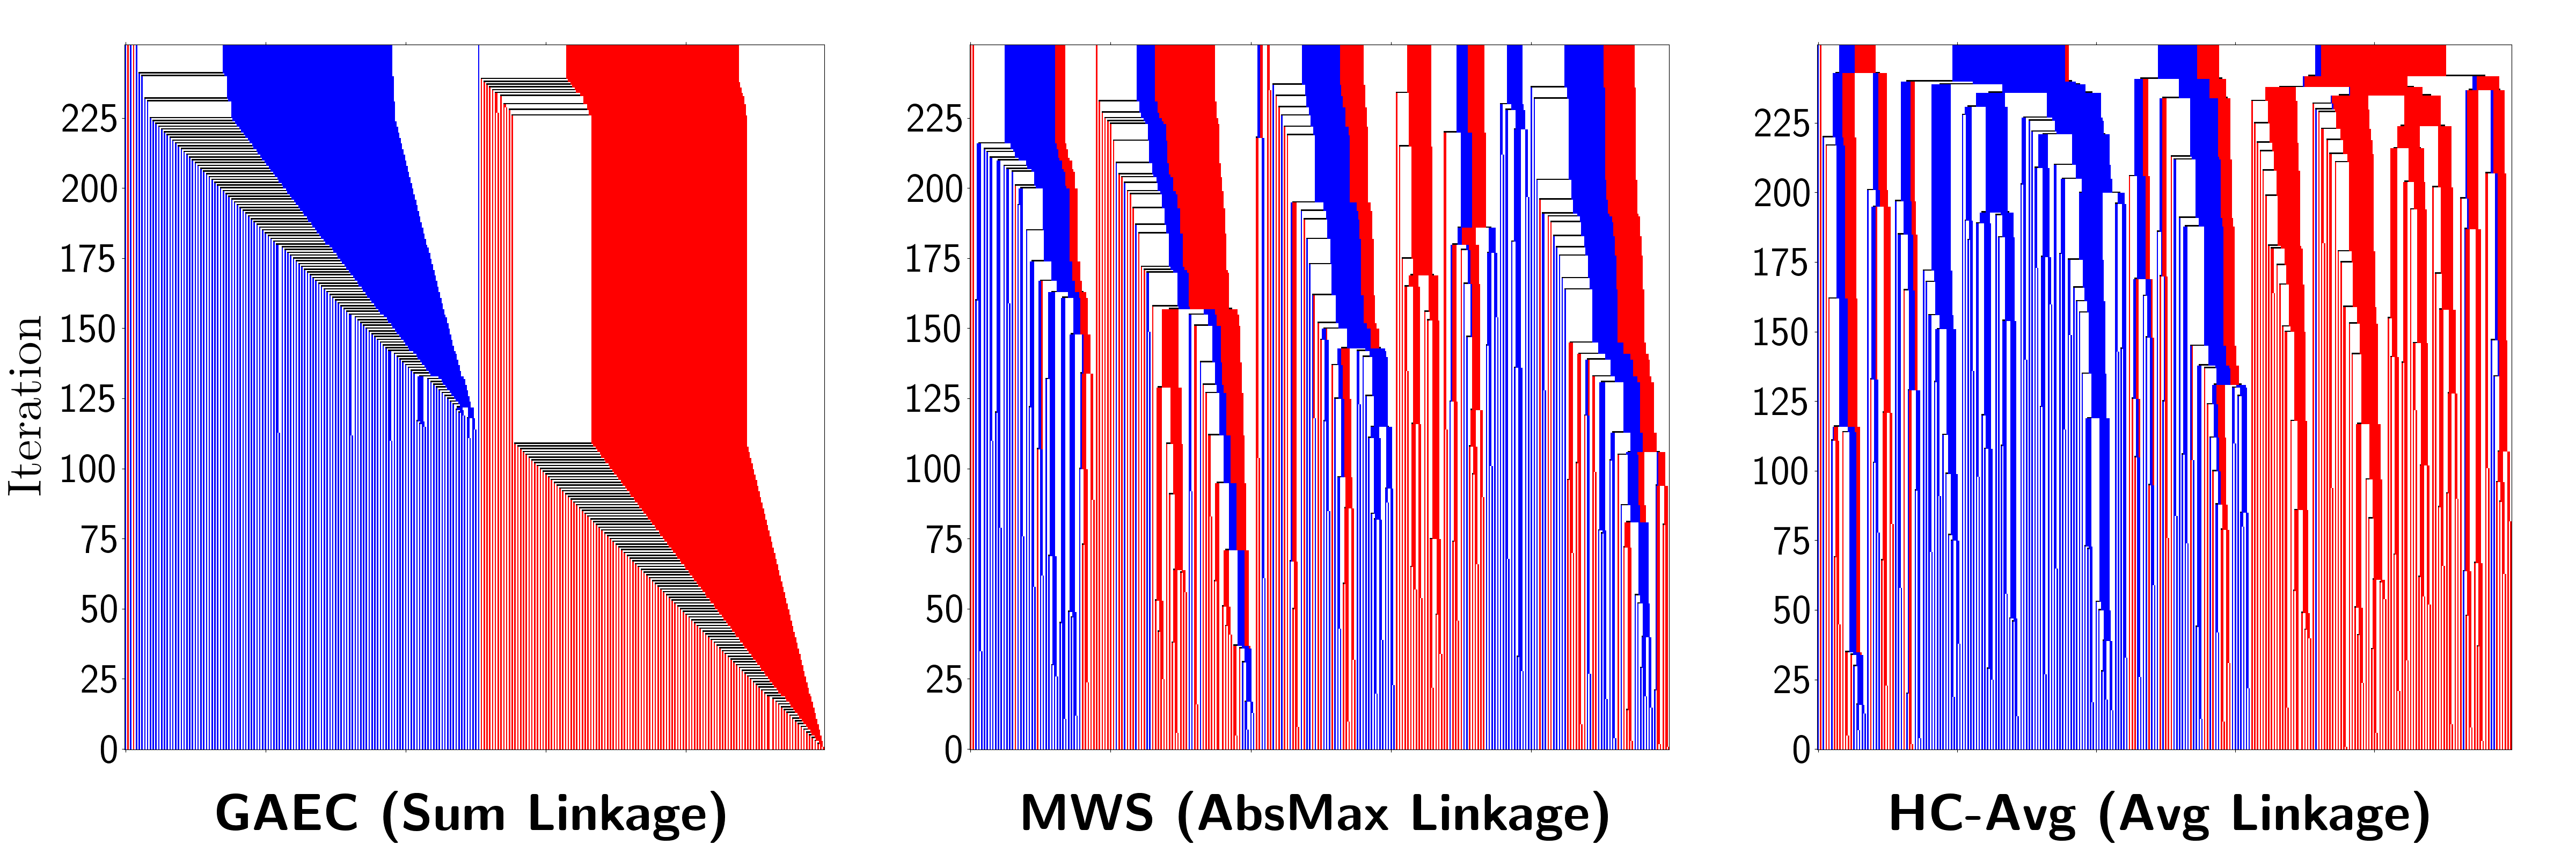
\includegraphics[width=0.48\textwidth,trim=80 10 60 0, clip]{./figs/dendrograms/new_agglo_order.png} % left bottom right top
\caption{Dendrograms built by three versions of \algname{} (GAEC, MWS, and HC-Avg) on a synthetic graph generated with SSBM ($N=250$, $p=0.05$, $\eta=0.1$, and $k=2$ communities of equal size).  Red and blue colors represent the true community of each initial node. At the top, dendrograms are truncated at the level of the final clustering $\Pi^*$ returned by \algname{} (y-axis shows the iteration number). \label{fig:dendrograms}}
\end{figure}






\textbf{Results on CREMI challenge} -- 
Table~\ref{tab:cremi_leaderboard} shows that the \emph{HCC-Avg} and \emph{HC-Avg} clustering algorithms achieve state-of-the-art performances on the CREMI challenge, when combined to the predictions of our CNN.
Most of the other entries (apart from \emph{LSI-Masks} \cite{bailoni2020proposal}) employ super-pixels based post-processing pipelines and cluster 3D-region-adjacency graphs. As we show in Table ~\ref{tab:scores_3drag}, using super-pixels considerably reduces the size of the clustering problem and, consequently, the post-processing time. 
However, our method operating directly on pixels (\emph{gridGraph+HCC-Avg}) achieves better performances than superpixel-based methods (\emph{3D-rag+HCC-Avg}) and does not require the parameter tuning necessary to obtain good super-pixels, which is usually highly dataset dependent.
The method \emph{3D-rag+LiftedMulticut} based on the lifted multicut formulation of \cite{beier2017multicut} (see details in Appendix) achieves the best scores overall, but it takes into account different information through the lifted edge weights that also depend on additional raw-data and super-pixel shape information. 
To scale up our method operating on pixels, we divided each test-volume into four sub-blocks, and then combined the resulting clusterings by running the algorithms again on the combined graph.
% Note that the test volumes of the challenge contain several imaging artifacts that make segmentation particularly challenging.
% However: handcrafted and dataset dependent, performs better, no

% Given By building a grid-graph from our CNN predictions  and solving a clustering problem with the \emph{HCC-Avg} and \emph{HC-Avg} algorithms, representing the best performing algorithms included in the proposed \algname{} framework, we achieve state-of-the-art performances on the competitive CREMI challenge (see Table~\ref{tab:cremi_leaderboard}). 

% To scale up the pixel-based aggSpecify that we divided samples into four blocks and then run the agglomeration again (moreover, run seeded WS to get rid of small segments).

% then \algname{} with cannot-link constraints shows a clear tendency to over-cluster. \\

% Superpixels are nice because they reduce runtime and represents the standard choices for connectomics (all bug LSI-Masks use some kind of similar form). But method is very dataset-dependent and require the user to set a series of parameters

% So far no other method was done from pixels


\begin{figure}
\centering
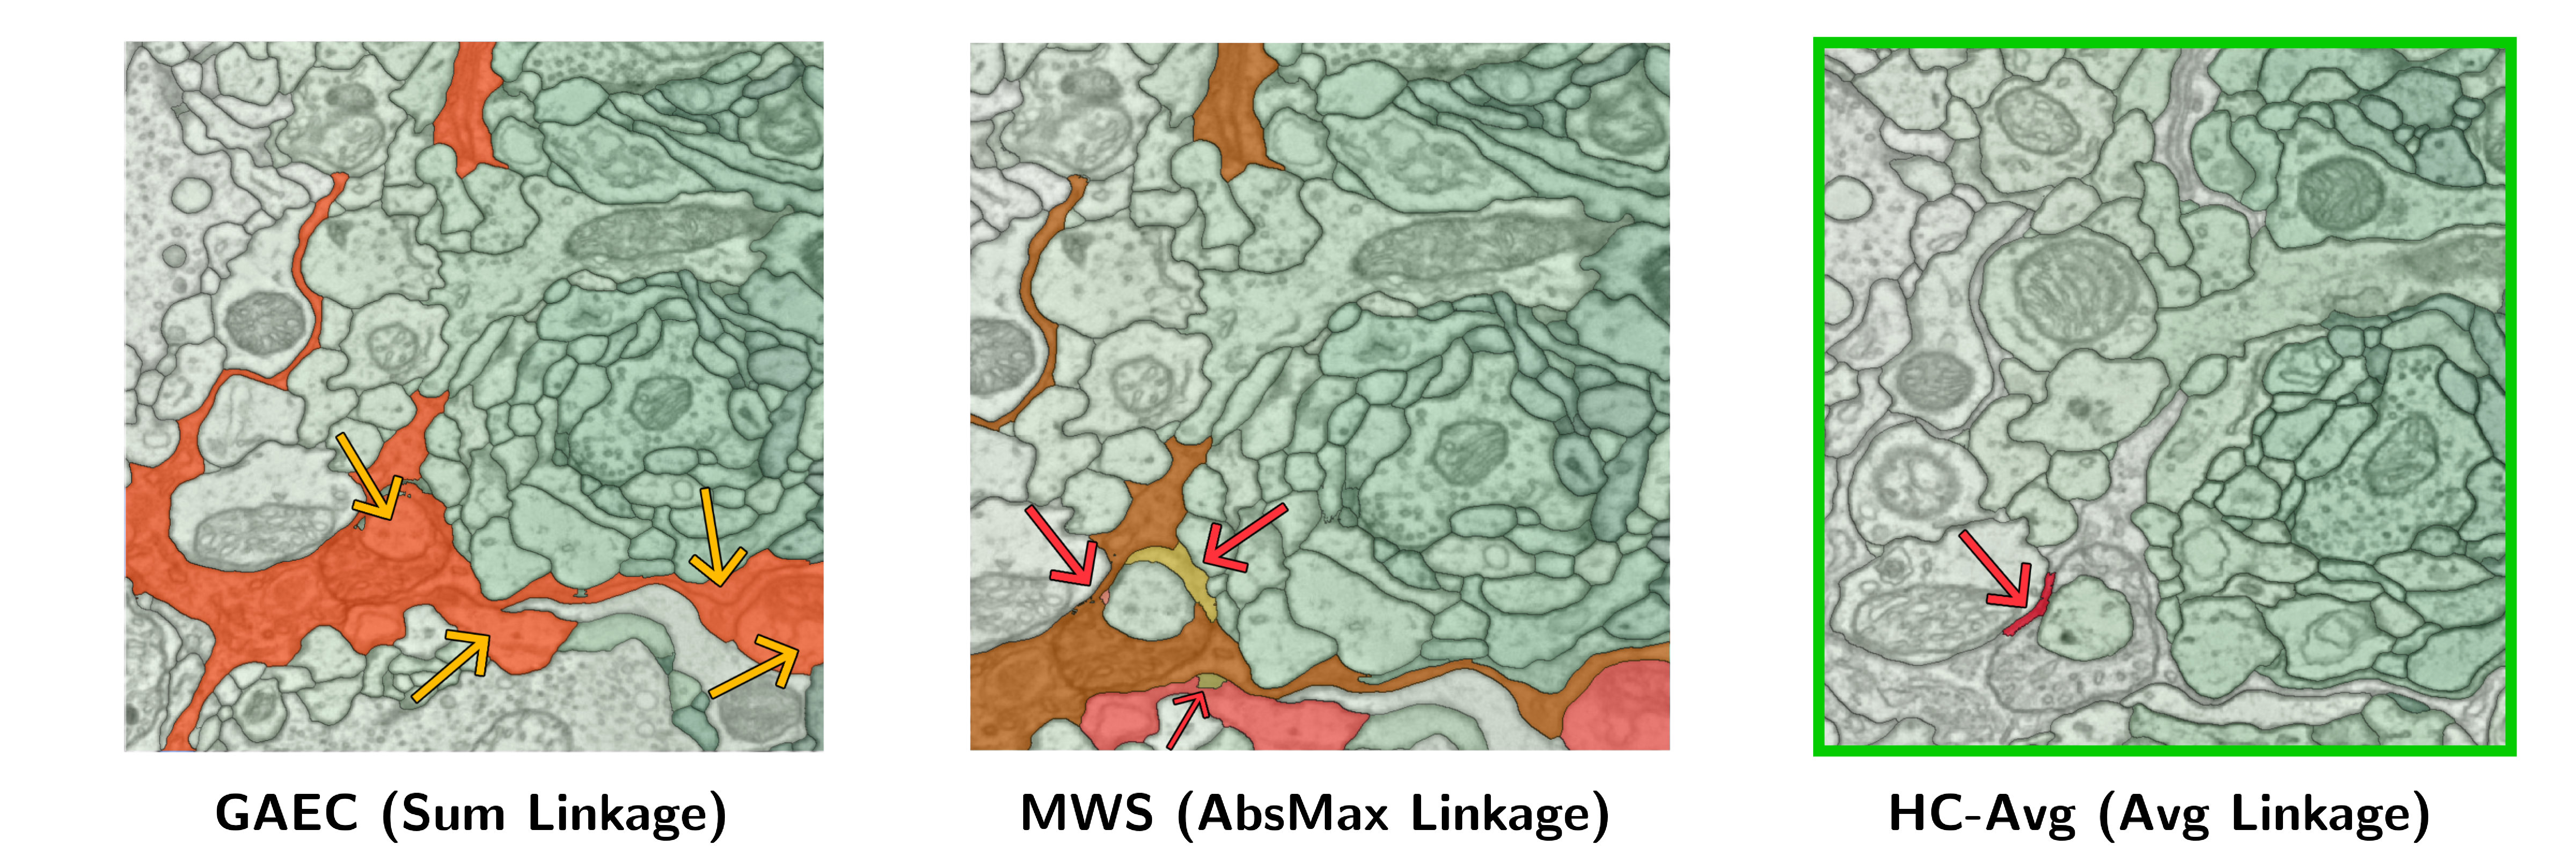
\includegraphics[width=0.48\textwidth,trim=90 10 60 0, clip]{./figs/comparison_GAEC_MWS_Avg.png} % left bottom right top
\caption{Failure cases of three versions of \algname{} on challenging parts of the CREMI dataset. \emph{Wrongly} segmented regions are highlighted in different warm colors. Red arrows point to wrongly split regions; yellow ones to merge errors. HC-Avg returned the best segmentation. Data is 3D, hence the same color could be assigned to parts of segments that appear disconnected in 2D.  
\label{fig:failure_cases}}
\end{figure}



% The competitive performance of this simple parameter-free algorithm is also reported in Table \ref{tab:results_cremi_test}, showing the current leader-board of the challenge: 


% Note that the test volumes contain several imaging artifacts that make segmentation particularly challenging. 
% and might profit from more robust edge statistics of super-pixel based approaches.

% and can also avoid errors that result from wrong superpixels that cannot be fixed during later agglomeration.
% In Appendix \ref{sec:appendix_exps_full_cremi}, we provide more details about how we scaled up \algname{} to the full datasets. 
% Appendix Table \ref{tab:extended_results_cremi} lists the performances and the run-times for all tested \algname{} linkage criteria.\\


% We first evaluate and compare the agglomerative clustering algorithms described in the generalized framework on the task of neuron segmentation in electron microscopy (EM) image volumes. This application is of key interest in connectomics, a field of neuro-science with the goal of reconstructing neural wiring diagrams spanning complete central nervous systems. Currently, only proof-reading or manual tracing yields sufficient accuracy for correct circuit reconstruction \cite{schlegel2017learning}, thus further progress is required in automated reconstruction methods.

% EM segmentation is commonly performed by first predicting 
% boundary pixels \cite{beier2017multicut,ciresan2012deep} or undirected affinities \cite{wolf2018mutex,lee2017superhuman,funke2018large}, which represent how likely it is for a pair of pixels to belong to the same neuron segment. 
% The affinities do not have to be limited to immediately adjacent pixels.
% Thus, similarly to \cite{lee2017superhuman}, we train a CNN to predict both short- and long-range affinities
% and use them as edge weights of a 3D grid graph, where each node represents a pixel/voxel of the volume image. 


